\documentclass[11pt]{article}

%%%%%%%%%%%%%%Include Packages%%%%%%%%%%%%%%%%%%%%%%%%%%
\usepackage{xcolor}
\usepackage{mathtools}
\usepackage[a4paper, total={6in, 8in}, margin=1.25in]{geometry}
\usepackage{amsmath}
\usepackage{amssymb}
\usepackage{paralist}
\usepackage{rsfso}
\usepackage{amsthm}
\usepackage{wasysym}
\usepackage[inline]{enumitem}   
\usepackage{hyperref}
\usepackage{tocloft}
\usepackage{titlesec}
\usepackage{colortbl}
%%%%%%%%%%%%%%%%%%%%%%%%%%%%%%%%%%%%%%%%%%%%%%%%%%%%%%%%



\begin{document}
\Large \noindent \textbf{Physics 1A Discussion (Week 2)}\\
\normalsize
Department of Physics and Astronomy, UCLA\\
\noindent\rule{8cm}{0.4pt}\\


\noindent\textbf{Problem}: A movie stuntwoman drops from a helicopter that is $30.0$ meters above the ground and moving with a constant velocity whose components are $10$\,m/s upward and $15$\,m/s towards the south. \\

(a) Neglect air resistance, where on the ground (relative to the position of the helicopter when she drops) should the stuntwoman have placed foam mats to break her fall?\\

\hfill\break
\hfill\break
\hfill\break
\hfill\break
\hfill\break
\hfill\break
\hfill\break
\hfill\break
\hfill\break

(b) Draw the $x$\,-\,$t$, $y$\,-\,$t$, $v_x$\,-\,$t$, and $v_y$\,-\,$t$ graphs of her motion.\\

\hfill\break
\hfill\break
\hfill\break
\hfill\break
\hfill\break
\hfill\break
\hfill\break
\hfill\break
\hfill\break
\hfill\break
\hfill\break
\hfill\break

(c) Compute the highest height that she could reach, $y_{\max}$. 






\newpage
\textbf{Solutions:}\\

(a) Since the stuntwoman drops (free falling) from the helicopter, she has an initial velocity $10\,$m upward and $15\,$m to the south. We have seen the kinematic equations last week, 
\begin{align*}
v_y = a_y t+ v_{i,y}\,,\qquad y = \frac{1}{2}a_y t^2 + v_{i,y} t + y_0
\end{align*}
for vertical motion and
\begin{align*}
v_x = a_x t+ v_{i,x}\,,\qquad 
x = \frac{1}{2}a_x t^2 + v_{i,x} t + x_0
\end{align*}
for horizontal (in this case, going south) motion.\\

\noindent\fbox{%
  \begin{minipage}{\dimexpr\linewidth-2\fboxsep-2\fboxrule}

\section*{Motion with constant acceleration}
The way that we obtain these two kinematic equations is the following: We start with a constant acceleration $a_y$ (or $a_x$ for the horizontal motion). Integrating once with respect to time we have the velocity,
\begin{align*}
v_y =\int a_y\, dt  = a_y t + v_{i,y}
\end{align*}
where $v_{i,y}$ is a constant (the $+C$ in your integration) indicating the initial velocity at time zero. Then integrating with respect to time again we obtain the position, 
\begin{align*}
y = \int v_y dt = \frac{1}{2}a_y t^2 + v_{i,y} t + y_0\,,
\end{align*}
where $y_0$ is another constant (another $+C$ from the integral) indicating the initial position. This gives the kinematic equation in vertical direction that we can find the position of the object at any given time $t$. Similar steps lead to the corresponding ones for motion in the horizontal direction. 

  \end{minipage}%
}

\hfill\break

Now, the acceleration in the vertical direction is $a_y = -9.8$\,m/s$^2$ because the only thing that affect the stuntwoman's motion is gravity. The acceleration in the horizontal direction is $a_x = 0$\,m/s$^2$ because we have neglected air resistance and gravity has no effect on horizontal motion. Initial position is $y_0 = 30$ meters and $x_0 = 0$ meters. Thus we have
\begin{align*}
y = -4.9 t^2 + 10 t + 30\,,\qquad\qquad
x = 15 t \,.
\end{align*}
When she reaches the ground, she reaches $y=0$ meters, so we can compute the time she gets to the ground by setting $y =0$ in the first equation, 
\begin{align*}
0  =-4.9 t^2 + 10 t + 30\,.
\end{align*}
Using quadratic equation and keep the positive time, we find
\begin{align*}
t = 3.697\,\text{s}\,.
\end{align*}
By this time, she has traveled
\begin{align*}
x = 15 \cdot 3.697 = 55.46\,\text{m}
\end{align*}
horizontally from where she drops. This tells us where on the ground to place the foam mat.\\

(c) To find the top of her trajectory, we want to find the maximum of the parabola
\begin{align*}
y= \frac{1}{2}a_y t^2 + v_{i,y} t + y_0\,.
\end{align*}
There are many ways to do this. Since this class is calculus based, we take the first derivative to find where $y$ attains its maximum, 
\begin{align*}
\frac{dy}{dt} = a_y t + v_{i,y} = 0\,,
\end{align*}
so we require
\begin{align*}
t = -\frac{v_{i,y}}{a_y}
\end{align*}
for $y$ being maximized. Thus we write
\begin{align*}
y_{\max} = \frac{1}{2}a_y \left(-\frac{v_{i,y}}{a_y}\right)^2 + v_{i,y} \left(-\frac{v_{i,y}}{a_y}\right) + y_0 = -4.9(10/9.8)^2 + 10(10/9.8) + 30 =35.1\,\text{m}\,. 
\end{align*}


(b) Here are the plots.
\begin{center}
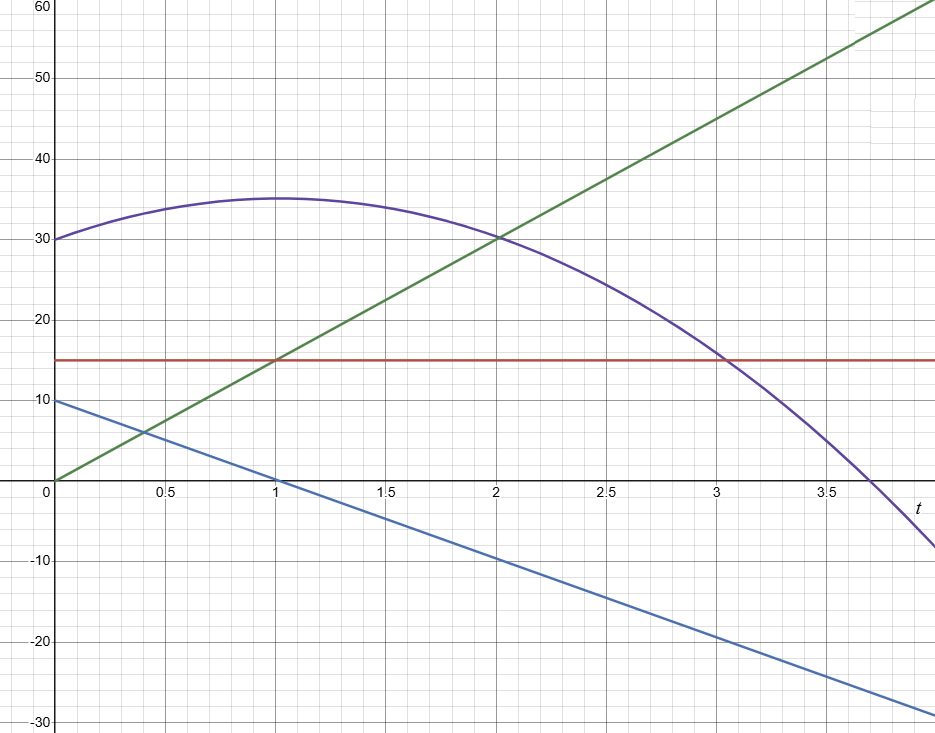
\includegraphics[scale=0.5]{wk2}
\end{center}
Purple: $y$\,-\,$t$ plot.
Green: $x$\,-\,$t$ plot.
Blue: $v_y$\,-\,$t$ plot.
Red: $v_x$\,-\,$t$ plot.\\

* I am being lazy here, you should also label the axes with the corresponding \underline{units} when plotting these. This is important for getting full credits for your plots.\\

\newpage
\noindent\fbox{%
  \begin{minipage}{\dimexpr\linewidth-2\fboxsep-2\fboxrule}

\section*{Circular motion}
Now instead of having $\vec{a} = (a_x,\,a_y)$ being fixed, we want $\vec{a}$ to be changing at all time (at least its direction) to obtain a circular motion. For describing some object moving in a circular path, we want to have 
\begin{align*}
r = \sqrt{x^2 + y^2} = \text{constant} \tag{*}
\end{align*}
being fixed (such that we obtain a perfect circular path with radius $r$). This is the only constraint that we want for circular motion. One might be tempted to start with the system of differential equations,
\begin{align*}
\vec{x} = (x,y)\qquad
\vec{v} =\left(\frac{dx}{dt}\,,\ \frac{dy}{dt}\right) \,,\qquad
\vec{a} =\left(\frac{d^2x }{dt^2}\,,\ \frac{d^2y}{dt^2}\right)\,, \tag{**}
\end{align*}
to obtain the equation of motion for the object, just like what we have done for describing motion with constant acceleration (integrate $\vec{a}$ to get $\vec{v}$ and integrate $\vec{v}$ to get $\vec{x}$). However, at this time, we want to solve this system (**) under the constraint (*), and it is very difficult to incorporate (*) into (**) using Cartesian coordinates. Thus the first step here is to write down (**) in polar coordinates instead, 
\begin{align*}
\vec{x} = (r,\theta)\,,\qquad
\vec{v} = \left(\frac{dr}{dt}\,,\
r\frac{d\theta}{dt}\right)\,,\qquad
\vec{a} = \left(\frac{d^2 r}{dt^2} - r \left( \frac{d\theta}{dt}\right)^2\,,\ 2\frac{dr}{dt}\frac{d\theta}{dt} + r\frac{d^2\theta}{dt^2}\right)\,.\tag{$\dagger$}
\end{align*}  
Now (*) literally states that $dr/dt = 0$ and $d^2r/dt^2 = 0$, which kill a lot of terms in ($\dagger$), leaving
\begin{align*}
\vec{x} = (r,\theta)\,,\qquad
\vec{v} = \left(0\,,\
r\frac{d\theta}{dt}\right)\,,\qquad
\vec{a} = \left(- r \left( \frac{d\theta}{dt}\right)^2\,,\  r\frac{d^2\theta}{dt^2}\right)\,.
\end{align*}
The radial component of $\vec{a}$ gives a \underline{requirement for maintaining such circular motion}, 
\begin{align*}
a_c = |a_r| = r\left( \frac{d\theta}{dt}\right)^2 = r\omega^2 = \frac{v_{t}^2}{r}\,, \tag{$\ddagger$}
\end{align*}
where I have defined the tangential speed $v_t$ of the object in circular motion,
\begin{align*}
v_t = r\frac{d\theta}{dt} = r\omega\,.
\end{align*}
As long as ($\ddagger$) holds (so that we have a circular motion), then you can find the exact location of the object at $(r,\theta)$, with
\begin{align*}
\theta = \int \omega \,dt\,,\qquad\text{where }\omega=\frac{d\theta}{dt} = \int \alpha \, dt =\int \frac{d^2\theta}{dt^2}\, dt\,.
\end{align*}
If we have a constant angular acceleration $\alpha$, we find 
\begin{align*}
\theta = \frac{1}{2}\alpha t^2 + \omega_i t + \theta_i\,.
\end{align*}
This is the complete story about circular motion, mathematically.  \end{minipage}%
}

\noindent\fbox{%
  \begin{minipage}{\dimexpr\linewidth-2\fboxsep-2\fboxrule}

For working on problems, for sure you don't need to re-derive these equations. The things that we expect you to be able to do are the followings:\begin{enumerate}
\item When we talk about circular motions, make sure that we have $a_c = v_t^2/r$, and be able to talk about what $a_c$ and $v_t$ are, including their directions ($a_c$ points towards the center of the circular path, $v_t$ is tangent to the circular path).
\item For circular motion, you should be able to compute $\theta$, $\omega$, or $\alpha$, when appropriate quantities are given, just like computing $(x,y)$ for the stuntwoman in today's discussion problem. 
\item You should be able to convert between the tangential quantities ($v_t$ and $a_t$) and angular quantities ($\omega$ and $\alpha$). You should know $v_t = r\omega$, and $a_t = r\alpha$. 
\end{enumerate}
  \end{minipage}%
}


\end{document}
